% Introduction
% ============

\chapter{Introduction}
\label{ch:introduction}

\section{Qu'est-ce que la calculabilité}
\label{sec:qu_est-ce_la_calculabilite}

\paragraph{}

La calculabilité c'est l'étude des limites de l'informatique. Il faut bien
faire attention à faire la différence entre les limites théoriques et les limites
pratiques. Pour la calculabilité, on s'occupe des limites théoriques alors que pour 
la complexité on s'occupe des limites pratiques. La complexité
détermine la frontière entre ce qui est faisable et infaisable en pratique.
La question principale de la calculabilité est: ``quels sont les problèmes qui peuvent
être résolus par un programme?''.  De manière informelle, un problème est dit calculable s'il existe un programme qui résout ce problème.  La caractéristique d'un problème calculable ne donne donc aucune 
autre information que de la preuve de l'existence d'un programme pour résoudre ce problème.  Mais lorsqu'un problème est non calculable, cela nous informe qu'il est inutile d'essayer d'écrire un programme pour résoudre ce problème; un tel programme n'existe pas!

\paragraph{} Le but est donc de tracer des frontières entre les programmes calculables,
non calculables et non calculables en pratique.

\subsection{Exemples de limites}
\label{subsec:exemples_limites}

De nombreuses limites existent en informatique, par exemple il est impossible de déterminer quand un programme se termine. Ou bien on ne peut pas déterminer qu'un programme est écrit sans bugs.

Mais des limites existent dans bien d'autres domaines que l'informatique. 
Par exemple dans plusieurs champs de la physique tel que la 
thermodynamique où des lois établissent que l'on ne peut créer de l'énergie à partir de rien.

\section{Notion de problème}
\label{sec:notion_de_probl_me}

\paragraph{}
Premièrement, on doit parler de la notion de problème.
Attention, il ne faut pas confondre un problème avec un programme.
Les caractéristiques d'un problème sont:

\begin{itemize}
	\item un problème est générique : il s'applique à un ensemble de données.
	\item pour chaque donnée particulière, il existe une réponse.
\end{itemize}
On représente un problème dans le cours par une fonction. Donc dans le cours,
la description d'un problème est équivalente à la description d'une fonction.
% paragraph  (end)
% section notion_de_probl_me (end)

\section{Notion de programme}
\label{sec:notion_de_programme}

Un programme est une ``procédure effective'', c'est-à-dire exécutable par une machine.
Il existe plein de formalismes permettant la description de ``procédure effective''.

% section notion_de_programme (end)

\section{Résultats principaux}
\label{sec:r_sultat_principaux}

\subsection{ Équivalence des langages de programmation}
\label{subsec:equivalence_des_langages_de_programmation}

Y a t-il de langage de programmation qui sont plus puissants que d'autres ? Tous les langages sont-ils équivalents ? 
\newline 
Il y a une équivalence entre langages en termes de calculabilité.  Lorsqu'un problème peut être résolu par un de ces langages, il peut alors être résolu par n'importe lequel autre.   
S'il existe un programme Java qui résout un problème, il existera aussi un programme C/C++, PHP, … qui peut résoudre le même problème. On parle d'une équivalence théorique.\\
D'un point de vue théorique ces langages s'appellent des langages complets. Ils permettent tous de résoudre les même problèmes.  Un problème est donc calculable indépendamment du langage utilisé. \\
D'un point de vue pratique on peut voir des différences (le programme sera plus court, s'écrire plus rapidement, le programme sera plus rapide, plus propre, plus fiable et encore d'autres critères).  Certains langages sont donc mieux adaptés que d'autres pour certains problèmes. 


\subsection{Existence de problèmes non calculables}
\label{subsec:existence_de_problemes_non_calculables}
	Problème non calculable : il existe des problèmes qui ne peuvent
		être résolus par un programme. Ex:
        détection de virus,
        équivalence de programme,
        déterminer si un polynôme à coefficients entiers a des racines entières, ...
	
% section r_sultat_principaux (end)

\subsubsection{Exemple: Détection de virus}
\label{subsubsec:detection_de_virus}
On veut déterminer si un programme P avec une entrée D est nuisible.

\textbf{Être nuisible:} Un programme est dit nuisible si son exécution a pour effet de contaminer d'autres programmes (par exemple: le programme va se recopier autre part). 

Spécification du programme \lstinline{detecteur(P,D)}:\\
\textbf{Préconditions :} un programme P et une donnée D\\
\textbf{Postconditions :} ``Mauvais'' si P(D) est nuisible,
		``Bon'' sinon.\\
Il faut aussi que \lstinline{detecteur} ne soit pas nuisible.

Faisons l'hypothèse qu'un programme \lstinline{detecteur(P,D)} existe et que celui-ci ne soit pas nuisible.  Sous cette hypothèse, on peut construire le programme  \lstinline{drole(P)} suivant.

\label{lst:detecteur_de_virus}
\begin{lstlisting}
drole(P)
if detecteur(P,P) = "Mauvais"
	then stop
else infecter un autre programme en y inserant P
\end{lstlisting}

Regardons si l'exécution de \lstinline|drole(drole)| est nuisible ou non.  
\begin{lstlisting}
drole(drole)
if detecteur(drole, drole) = "Mauvais"
	then stop
else infecter un autre programme en y inserant drole
\end{lstlisting}

\begin{itemize}
	\item Supposons que \lstinline|drole(drole)| soit nuisible.
      Lorsqu'on exécute, \lstinline|drole(drole)|
      \lstinline|detecteur(drole,drole)| n'infecte rien car \lstinline|detecteur| n'est pas nuisible.
      Comme \lstinline|detecteur| retourne ``Mauvais'',
      le programme s'arrête.
      Rien a donc été infecté, ce qui est contradictoire avec le fait que \lstinline|drole(drole)| est nuisible.
	\item Si par contre il n'est pas nuisible alors \lstinline|detecteur(drole,drole)|
      ne va pas retourner Mauvais et on va arriver dans le \lstinline|else|.
      On a donc infecter un autre programme que qui contredit le fait que \lstinline|drole(drole)| n'est pas nuisible.
\end{itemize}

On a donc une contradiction dans tous les cas, ce qui implique que le programme \lstinline|drole| ne peut pas
exister. Vu que la seule hypothèse que nous avons formulée pour écrire le programme \lstinline|drole| est que \lstinline|detecteur| (non nuisible) existe, 
cela implique que le programme \lstinline|detecteur| (non nuisible) n'existe pas non plus.
% paragraph  (end)
% subsubsection d_tection_de_virus (end)

\subsection{ Existence de problèmes intrinsèquement complexes}
\label{subsec:existence_de_problemes_intrinsequement_complexes}

Un problème intrinsèquement complexe et un problème dont le meilleur algorithme n'a pas de complexité polynomiale, mais une complexité exponentielle ou pire.  Peu importe les évolutions technologiques, un problème exponentiel ne peut et ne pourra être résolu que pour des données de petite taille.  Un exemple est le problème du voyageur de commerce qui doit rechercher le trajet le plus court pour relier $n$ villes.  Pour un problème intrinsèquement complexe, lorsqu'un ordinateur est $n$ fois plus rapide,  la taille des problèmes pouvant être résolus en temps raisonnable est incrémentée d'une petite valeur (voir le tableau ci-dessous).

Supposons un ordinateur actuel sachant faire 100 millions d'instructions par seconde ($100$ Mips) et que le traitement d'un élément nécessite 100 instructions machines.  Dénotons $N_i$  la taille du ``plus grand'' exemple dont la solution peut-être calculée en 1 heure de temps calcul.	

\begin{center}
	$\begin{array}{|c||c|c|c|}
		\hline
		\text{Complexité} & \text{Ordinateur actuel} & \text{100x plus rapide} & \text{1000x plus rapide} \\
		\hline
		n & N_1 = 3.6\times 10^9 & 100 N_1 & 1000 N_1 \\
		n^2 & N_2 = 6\times 10^5 & 10 N_2 & 31.6 N_2 \\
		n^3 & N_3 = 1530 & 4.64 N_3 & 10 N_3 \\
		n^5 & N_4 = 81 & 2.5 N_4 & 3.98 N_4 \\
		\hline
		2^n & N_5 = 31 & N_5 + 6 & N_5 + 10 \\
		3^n & N_6 = 20 & N_6 + 4 & N_6 + 6 \\
		\hline
	\end{array}$
\end{center}
		
\section{Objectifs calculabilité et complexité}
\label{sec:objectifs_calculabilite_et_complexite}

La figure Fig(\ref{cal_non_cal}) illustre la frontière entre les problèmes non calculables (il n'existe pas un programme) et calculables (il existe un programme).  Parmi les problèmes calculables il y a ceux qui le sont en pratiques (pas exponentiels) et ceux qui ne sont pas calculables en pratique. 
\begin{figure}[h]
	\centering
	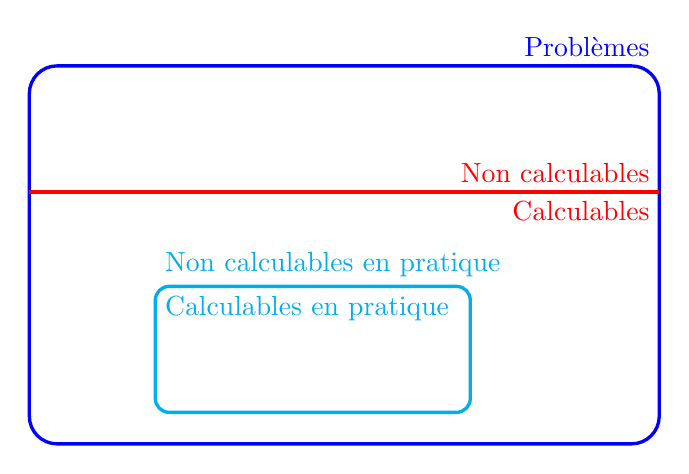
\begin{tikzpicture}[scale=0.8]
	\draw[very thick,blue,rounded corners=10pt]  (0,0) rectangle (10,6);
	\draw[very thick,red]   (0,4) -- (10,4);
	\draw[very thick,cyan,rounded corners=5pt] (2,0.5) rectangle (7,2.5);
	\draw[blue]  (10,6)  node[above left] {Problèmes};
	\draw[red]   (10,4)  node[above left] {Non calculables};
	\draw[red]   (10,4)  node[below left] {Calculables};
	\draw[cyan] (2,2.5) node[above right] {Non calculables en pratique};
	\draw[cyan] (2,2.5) node[below right] {Calculables en pratique};
	\end{tikzpicture}
	\caption{ Problèmes calculables / non calculables }
	\label{cal_non_cal}
\end{figure}

L'intérêt de la calculabilité est de savoir quels problèmes sont calculables ou lesquels ne le sont pas.  Si un problème est non calculable, il est alors inutile  d'essayer de résoudre ce problème.  Si le problème est calculable mais intrinsèquement complexe, il est inutile d'envisager un algorithme permettant de résoudre des problèmes de grande taille.  
Face à un problème non calculable ou intrinsèquement complexe,  on peut essayer de relâcher le problème pour le rendre calculable ou de complexité polynomiale.  Une solution à ce problème relâché peut par exemple être une approximation du problème initial.  
% section introduction (end)Introduction
